\subsection{線形系のリアプノフ安定性}

固有値や伝達関数の極による判定は線形時不変系に有効であるが、同じ安定性を二次形式などのスカラー関数の減少としても表現できる。ここでは内部安定性、すなわち $\dot{x}=Ax$ の原点の漸近安定性を、Lyapunov の直接法で判定する。平衡点 $x=0$ に対し、正定値関数 $V(x)$ があり
\begin{equation}
  V(x)>0\quad(x\ne0),\qquad V(0)=0
\end{equation}
を満たすとする。さらに軌道に沿った微分
\begin{equation}
  \dot{V}(x)=\frac{\pp V}{\pp x}f(x)
\end{equation}
が負定値なら、平衡点は漸近安定である。

線形系 $\dot{x}=Ax$ では、二次形式
\begin{equation}
  V(x)=x^\T P x,\qquad P=P^\T>0
\end{equation}
を考える。微分は
\begin{equation}
  \dot{V}=x^\T(A^\T P+PA)x
\end{equation}
である。任意の正定値 $Q$ に対して
\begin{equation}
  A^\T P+PA=-Q
\end{equation}
を満たす $P>0$ が存在すれば、$A$ は安定である。このリアプノフ方程式は、次に扱う LQR の価値関数へそのままつながる。

正定値行列は、ベクトルの重み付き大きさを作る行列である。$P>0$ なら $x^\T P x$ は $x\ne0$ で常に正になる。半正定値 $P\ge0$ では 0 になる方向が残る。評価関数や共分散行列で正定値性が重要になるのは、距離や不確かさを破綻なく測るためである。

\begin{figure}[tb]
\centering
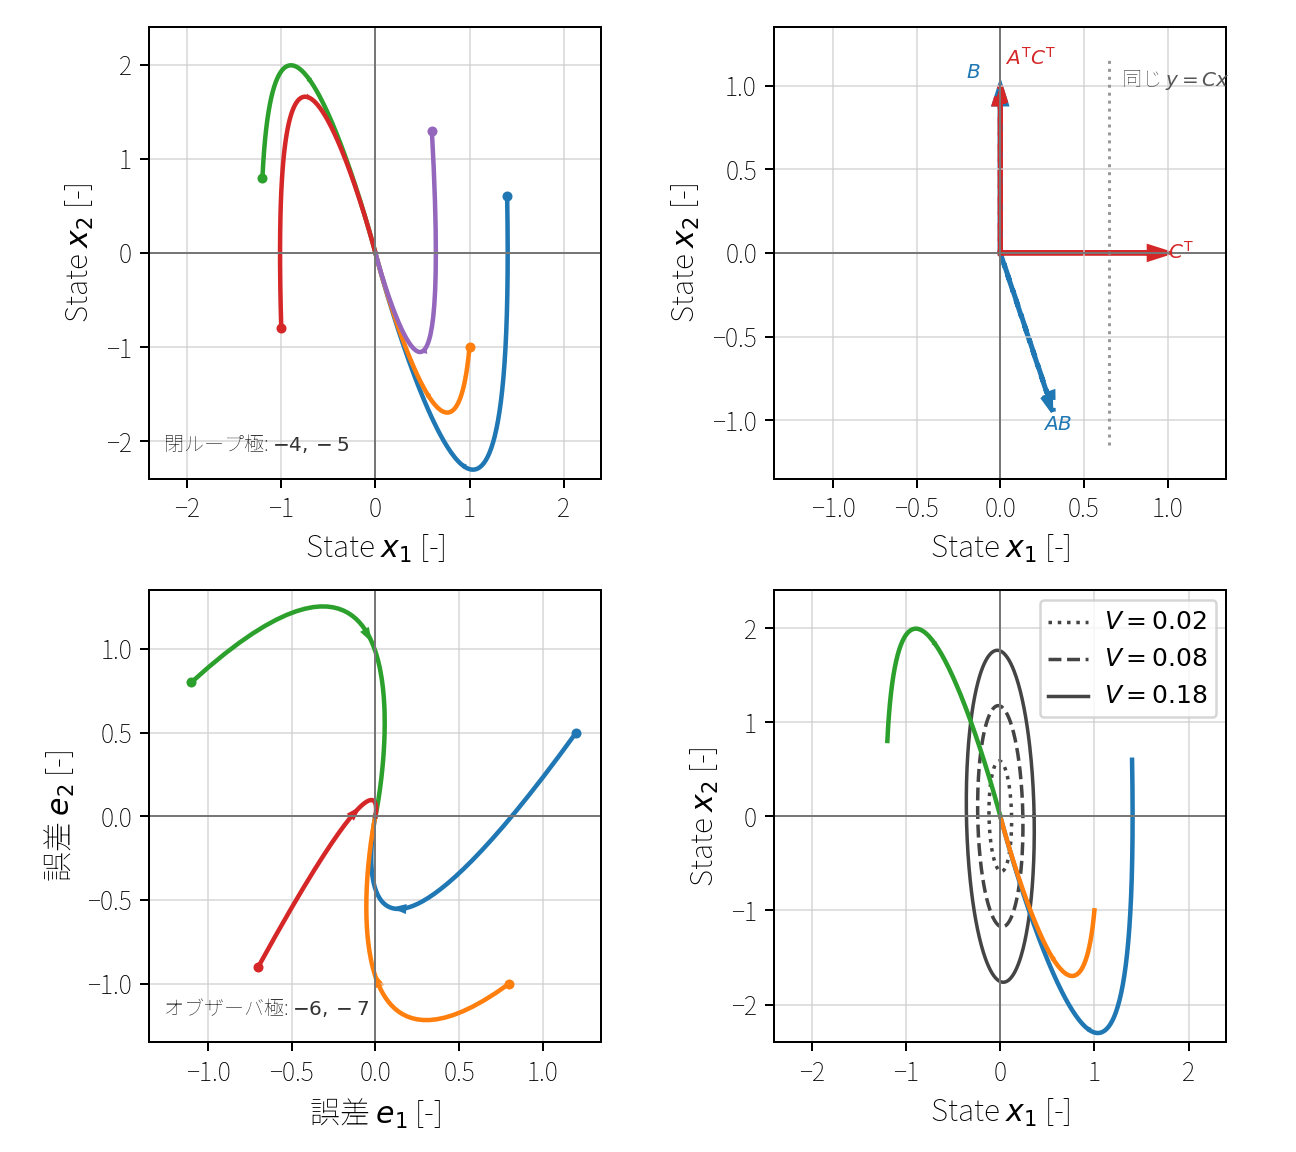
\includegraphics[width=0.94\linewidth,bb=0 0 1296 1152]{figures/state_space_geometry_examples.png}
\caption{二状態モデル $A=\left[\begin{smallmatrix}0&1\\-2&-3\end{smallmatrix}\right]$、$b=\left[\begin{smallmatrix}0&1\end{smallmatrix}\right]^\T$、$C=\left[\begin{smallmatrix}1&0\end{smallmatrix}\right]$ に対する状態空間の幾何。左上は $K=\left[\begin{smallmatrix}18&6\end{smallmatrix}\right]$ による閉ループ軌道、右上は可制御方向 $B,AB$ と可観測方向 $C^\T,A^\T C^\T$、左下は $L=\left[\begin{smallmatrix}10&10\end{smallmatrix}\right]^\T$ による推定誤差軌道、右下は $A-bK$ に対する $V=x^\T Px$ のレベル集合を示す。}
\label{fig:state-space-geometry-examples}
\end{figure}

図\ref{fig:state-space-geometry-examples} の右下では、閉ループ軌道が楕円の外側から内側へ横切っている。これは $\dot{V}=-x^\T Qx<0$ が、各軌道に沿って $V$ の値を単調に減らすことを幾何的に表している。左上の閉ループ軌道と左下の推定誤差軌道を比べると、制御極とオブザーバ極を別々に配置しても、どちらも原点へ向かう二次元の流れとして確認できる。

\begin{practice}[状態空間の幾何と信号経路の確認]
図\ref{fig:state-space-geometry-examples} の右上で、$B$ と $AB$ が一次独立であること、および $C$ と $CA$ が一次独立であることを、対応する可制御行列と可観測行列のランク計算で確認せよ。さらに、図\ref{fig:state-feedback-block} と図\ref{fig:observer-separation-block} の信号名を用いて、$r_u=0$ のときの閉ループ状態方程式と推定誤差方程式をそれぞれ書き出せ。
\end{practice}

\subsection{状態空間の式変形を省略しない}

\begin{theorem}[行列指数関数による解公式]
線形時不変系 $\dot{x}=Ax+Bu$ の解は
\begin{equation}
  x(t)=e^{At}x(0)+\int_0^t e^{A(t-\tau)}Bu(\tau)\,\dd\tau
\end{equation}
である。
\end{theorem}

\begin{derivation}
まず $u=0$ のとき、$x(t)=e^{At}x(0)$ とおく。行列指数関数の微分公式
\begin{equation}
  \frac{\dd}{\dd t}e^{At}=Ae^{At}
\end{equation}
より
\begin{equation}
  \dot{x}(t)=Ae^{At}x(0)=Ax(t)
\end{equation}
である。次に入力がある場合、定数変化法として $x(t)=e^{At}z(t)$ とおく。微分すると
\begin{align}
  \dot{x}(t)&=Ae^{At}z(t)+e^{At}\dot{z}(t),\\
  Ax(t)+Bu(t)&=Ae^{At}z(t)+Bu(t).
\end{align}
両者を等しいとおくと
\begin{equation}
  e^{At}\dot{z}(t)=Bu(t)
\end{equation}
である。左から $e^{-At}$ を掛けて
\begin{equation}
  \dot{z}(t)=e^{-At}Bu(t)
\end{equation}
となる。時刻 $0$ から $t$ まで積分すると
\begin{equation}
  z(t)=z(0)+\int_0^t e^{-A\tau}Bu(\tau)\,\dd\tau.
\end{equation}
$x(0)=z(0)$ なので
\begin{align}
  x(t)&=e^{At}x(0)+e^{At}\int_0^t e^{-A\tau}Bu(\tau)\,\dd\tau\\
  &=e^{At}x(0)+\int_0^t e^{A(t-\tau)}Bu(\tau)\,\dd\tau.
\end{align}
\end{derivation}

\begin{theorem}[Lyapunov の直接法]
平衡点 $x=0$ の近くで、正定値関数 $V(x)$ が存在し、軌道に沿った微分 $\dot{V}(x)$ が負定値なら、その平衡点は漸近安定である。
\end{theorem}

線形系で $V=x^\T Px$ と置くとき、$P=P^\T>0$ なら $V$ は正定値である。微分は積の微分公式より
\begin{align}
  \dot{V}
  &=\dot{x}^\T Px+x^\T P\dot{x}\\
  &=(Ax)^\T Px+x^\T P(Ax)\\
  &=x^\T A^\T Px+x^\T PAx\\
  &=x^\T(A^\T P+PA)x.
\end{align}
ここで $A^\T P+PA=-Q$、$Q>0$ なら
\begin{equation}
  \dot{V}=-x^\T Qx<0\quad(x\ne0)
\end{equation}
なので、Lyapunov の直接法より原点は漸近安定である。
